\documentclass[10pt]{article}

\usepackage{graphicx}
\usepackage{color}
\usepackage{tikz}
\usepackage{pgfplots}
\usepackage{pgf-umlsd}
\usepackage{ifthen}
\usepackage[a0paper,landscape]{geometry}
\begin{document}

\begin{figure}
\centerline
	\noindent\resizebox{\textwidth}{!}{
	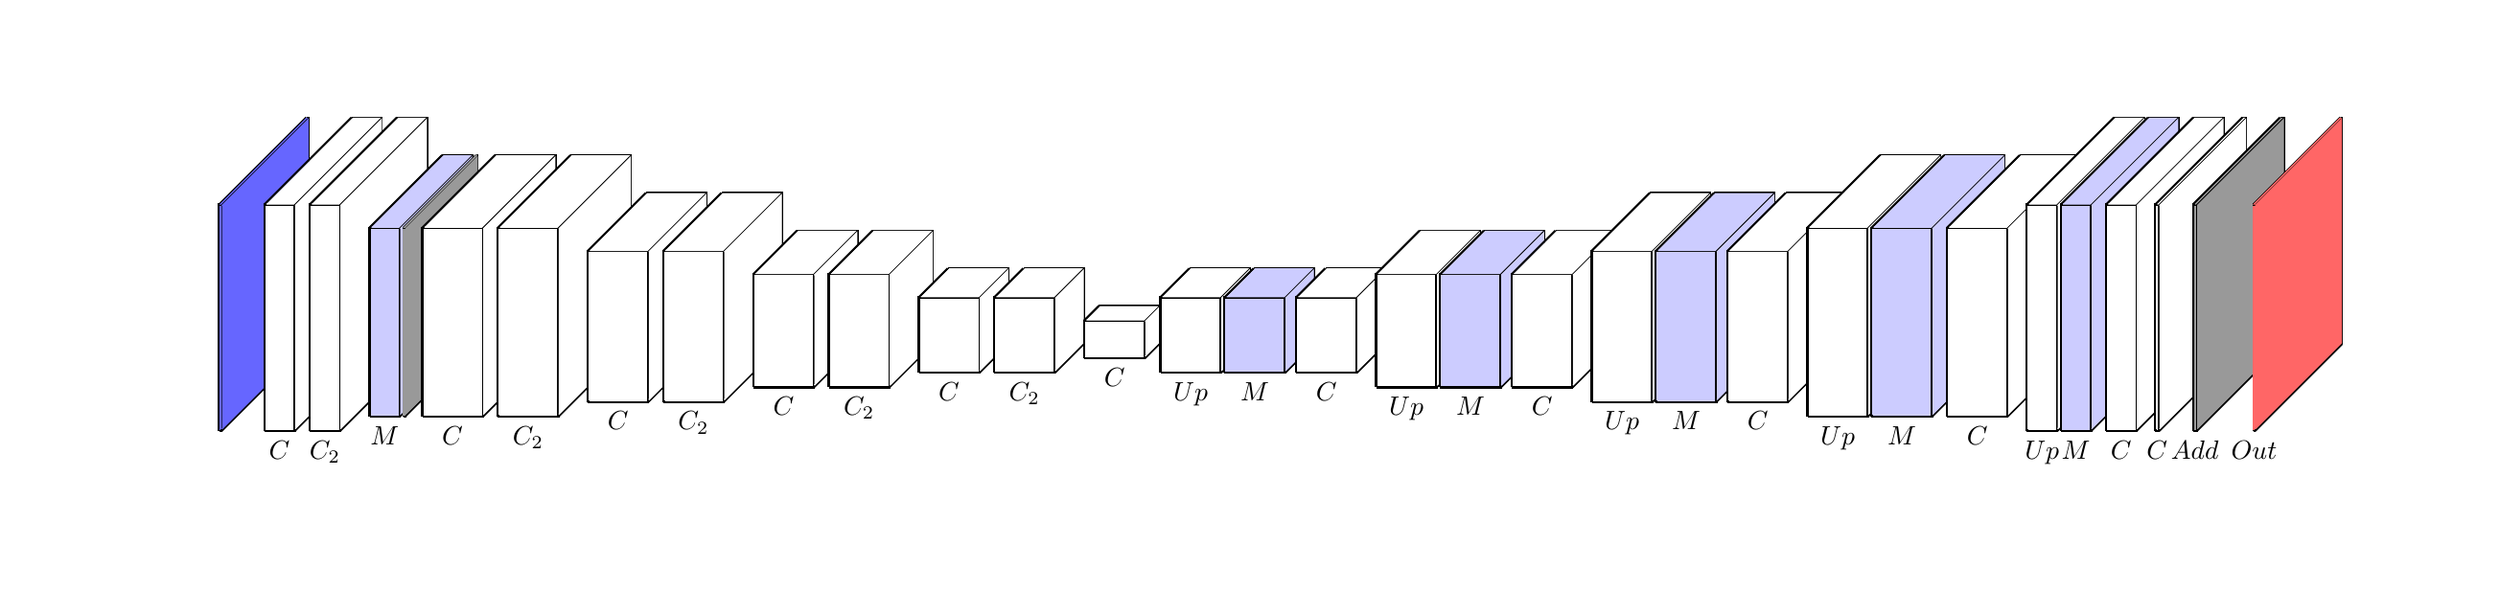
\begin{tikzpicture}
		\draw[use as bounding box, transparent] (-8.2,-3.2) rectangle (24.2, 4.2);

		% Define the macro.
		% 1st argument: Height and width of the layer rectangle slice.
		% 2nd argument: Depth of the layer slice
		% 3rd argument: X Offset --> use it to offset layers from previously drawn layers.
		% 4th argument: Options for filldraw.
		% 5th argument: Text to be placed below this layer.
		% 6th argument: Y Offset --> Use it when an output needs to be fed to multiple layers that are on the same X offset.

		\newcommand{\networkLayer}[6]{
			\def\a{#1} % Used to distinguish input resolution for current layer.
			\def\b{0.02}
			\def\c{#2} % Width of the cube to distinguish number of input channels for current layer.
			\def\t{#3} % X offset for current layer.
			\def\d{#4} % Y offset for current layer.

			% Draw the layer body.
			\draw[line width=0.3mm](\c+\t,0,\d) -- (\c+\t,\a,\d) -- (\t,\a,\d);                                                      % back plane
			\draw[line width=0.3mm](\t,0,\a+\d) -- (\c+\t,0,\a+\d) node[midway,below] {#6} -- (\c+\t,\a,\a+\d) -- (\t,\a,\a+\d) -- (\t,0,\a+\d); % front plane
			\draw[line width=0.3mm](\c+\t,0,\d) -- (\c+\t,0,\a+\d);
			\draw[line width=0.3mm](\c+\t,\a,\d) -- (\c+\t,\a,\a+\d);
			\draw[line width=0.3mm](\t,\a,\d) -- (\t,\a,\a+\d);

			% Recolor visible surfaces
			\filldraw[#5] (\t+\b,\b,\a+\d) -- (\c+\t-\b,\b,\a+\d) -- (\c+\t-\b,\a-\b,\a+\d) -- (\t+\b,\a-\b,\a+\d) -- (\t+\b,\b,\a+\d); % front plane
			\filldraw[#5] (\t+\b,\a,\a-\b+\d) -- (\c+\t-\b,\a,\a-\b+\d) -- (\c+\t-\b,\a,\b+\d) -- (\t+\b,\a,\b+\d);

			% Colored slice.
			\ifthenelse {\equal{#5} {}}
			{} % Do not draw colored slice if #4 is blank.
			{\filldraw[#5] (\c+\t,\b,\a-\b+\d) -- (\c+\t,\b,\b+\d) -- (\c+\t,\a-\b,\b+\d) -- (\c+\t,\a-\b,\a-\b+\d);} % Else, draw a colored slice.
		}

		% INPUT
		\def\sb{4}
		%\node[] (input image) at (-\sb -4.0,0.6) {\includegraphics[height=35mm]{lenna.png}};

		\networkLayer{3.0}{0.03}{-0.5-\sb}{0.0}{color=blue!60}{}

		% ENCODER
		\networkLayer{3.0}{0.4}{0.1-\sb}{0.0}{color=white}{$C$}    % S1
		\networkLayer{3.0}{0.4}{0.7-\sb}{0.0}{color=white}{$C_{2}$}    % S2
		
		\networkLayer{2.5}{0.4}{1.3-\sb}{0.0}{color=blue!20}{$M$}        % concat
		\networkLayer{2.5}{0.02}{1.75-\sb}{0.0}{color=gray!80}{}
		\networkLayer{2.5}{0.8}{2.0-\sb}{0.0}{color=white}{$C$}        % S3
		\networkLayer{2.5}{0.8}{3.0-\sb}{0.0}{color=white}{$C_{2}$}        % S4
		\networkLayer{2.0}{0.8}{4.0-\sb}{0.0}{color=white}{$C$}    % S5
		\networkLayer{2.0}{0.8}{5.0-\sb}{0.0}{color=white}{$C_{2}$}        % S2
		\networkLayer{1.5}{0.8}{6.0-\sb}{0.0}{color=white}{$C$}    % S1
		\networkLayer{1.5}{0.8}{7.0-\sb}{0.0}{color=white}{$C_{2}$}        % S2
		\networkLayer{1.0}{0.8}{8.0-\sb}{0.0}{color=white}{$C$}    % S1
		\networkLayer{1.0}{0.8}{9.0-\sb}{0.0}{color=white}{$C_{2}$}
		\networkLayer{0.5}{0.8}{10.0-\sb}{0.0}{color=white}{$C$}    % S1
		
		        % S2

		% DECODER
		\def\dc{11.2}
		\def\w{0.8}
		\def\ds{0.05}
		\def\dd{0.2}

		\networkLayer{1.0}{0.8}{\dc-\sb}{0.0}{color=white}{$Up$} % S1
		\networkLayer{1.0}{0.8}{\dc+\w +\ds-\sb}{0.0}{color=blue!20}{$M$}
		\networkLayer{1.0}{0.8}{\dc+\w+\w-\sb+\dd }{0.0}{color=white}{$C$} 
		\def\dcn{\dc+\w+\w+\dd+\w+\dd+ \ds}
		\networkLayer{1.5}{0.8}{\dcn-\sb+ \dd}{0.0}{color=white}{$Up$} % S1
		\networkLayer{1.5}{0.8}{\dcn+\w-\sb+ \ds+ \dd}{0.0}{color=blue!20}{$M$}
		\networkLayer{1.5}{0.8}{\dcn+\w+\w-\sb+\dd +\dd}{0.0}{color=white}{$C$} 
		\def\dcnn{\dcn+\w+\w+\dd +\w +\dd+ \ds+ \dd}
		\networkLayer{2.0}{0.8}{\dcnn-\sb+ \dd}{0.0}{color=white}{$Up$} % S1
		\networkLayer{2.0}{0.8}{\dcnn+\w-\sb+ \ds+ \dd}{0.0}{color=blue!20}{$M$}
		\networkLayer{2.0}{0.8}{\dcnn+\w+\w-\sb+\dd+ \dd}{0.0}{color=white}{$C$} 
		\def\dcnnn{\dcnn+\w+\w+\dd+\w+\dd+ \ds+ \dd}
		\networkLayer{2.5}{0.8}{\dcnnn-\sb+ \dd}{0.0}{color=white}{$Up$} % S1
		\networkLayer{2.5}{0.8}{\dcnnn+\w-\sb+ \ds+ \dd}{0.0}{color=blue!20}{$M$}
		\networkLayer{2.5}{0.8}{\dcnnn+\w+\w-\sb+\dd+ \ds+\dd}{0.0}{color=white}{$C$} 
		\def\dcnnnn{\dcnnn+\w+\w+\dd+\w+\dd+ \ds+ \dd}
		\networkLayer{3.0}{0.4}{\dcnnnn-\sb+ \dd+0.05}{0.0}{color=white}{$Up$} % S1
		\networkLayer{3.0}{0.4}{\dcnnnn+0.4-\sb+ \ds+ \dd+0.05}{0.0}{color=blue!20}{$M$}
		\networkLayer{3.0}{0.4}{\dcnnnn+0.4+0.4-\sb+\dd+\ds+ \dd+0.05}{0.0}{color=white}{$C$}
		\networkLayer{3.0}{0.05}{\dcnnnn+0.4+0.4-\sb+\dd+ \dd+0.4+\dd+0.1+0.05}{0.0}{color=white}{$C$}
		\networkLayer{3.0}{0.05}{\dcnnnn+0.4+0.4-\sb+\dd+ \dd+0.4+\dd+0.1+0.3+\dd + \ds}{0.0}{color=gray!80}{$Add$}
		\networkLayer{3.0}{0.02}{\dcnnnn+0.4+0.4-\sb+\dd+ \dd+0.4+\dd+0.1+0.3+\dd+0.25 +\dd +\dd+\dd}{0.0}{color=red!60}{$Out$}
		
		

		% OUTPUT
		
		%\node[] (output image) at (\dcnnnn+0.4+0.4-\sb+\dd+ \dd+0.4+\dd+0.1+0.3+\dd+0.25 +\dd +\dd+\dd+1.75,0.6) {\includegraphics[height=35mm]{vermeer.jpg}};


	\end{tikzpicture}
	}
	
	\label{fig:cnn}
\end{figure}

\end{document}
\grid
